\pagestyle{fancy}
\fancyhf{}
\fancyhead[L]{PLL implementation}


\pagestyle{fancy}
\fancyhf{} % Clear all header and footer fields
\renewcommand{\headrulewidth}{1.5pt} 
% Define custom color for rules
\definecolor{myrulecolor}{RGB}{94,31,31}
\renewcommand{\headrule}{%
    {\color{myrulecolor}\hrule width\headwidth height\headrulewidth \vskip-\headrulewidth}
}
\fancyhead[L]{Data Converters In VLSI Systems} % Left-aligned header
\fancyhead[R]{\makebox[\textwidth][r]{\textbf{\nouppercase{\leftmark}}}} % Right-alig

\fancyfoot[L]{\textbf{Department of Electronics and Communication, UVCE}}
% \fancyfoot[C]{\textbf{Jan 2025 – Apr 2025}} % Center: Semester dates
\fancyfoot[R]{\textbf{Page \thepage}} % Right side: Page number
\renewcommand{\footrulewidth}{1.5pt}
\renewcommand{\footrule}{%
    {\color{myrulecolor}\hrule width\headwidth height\footrulewidth \vskip-\footrulewidth}
}
% Define a custom page style for section pages
\fancypagestyle{chapterstyle}{
        \fancyhf{} % Clear all header and footer fields
        \renewcommand{\headrulewidth}{0pt} 
        \fancyfoot[L]{\textbf{Department of ECE}} % Left side: Department name
%   \fancyfoot[C]{\textbf{Jan 2025 – Apr 2025}} % Center: Semester dates
        \fancyfoot[R]{\textbf{Page \thepage}} % Right side: Page number
}
\chapter{Introduction}
Data conveters are systems that convert analog signals to digital signals and digital signals to analog signals. These converters are termed as DACs (Digital to Analog Converters) and ADCs (Analog to Digital Converters). The
conversion of signals is essential in modern days as most of the systems are digital in nature. 
The conversion from Analog to Digital is majorly done by Quantizaion and Sampling. The quantization is the process of mapping a large set of input values to a smaller set of output values. The sampling is the process of converting a continuous signal into a discrete signal by taking samples at regular intervals.
The conversion from Digital to Analog is done by reconstructing the signal from the digital values. The reconstruction is done by using various techniques such as interpolation, filtering, etc
The figure \ref{fig:digital_analog_conversion} shows the conversion of digital signals to analog signals and vice versa. The digital signal are represented by discrete values, while the analog signals are represented by . 
\begin{figure}[H]
    \centering
    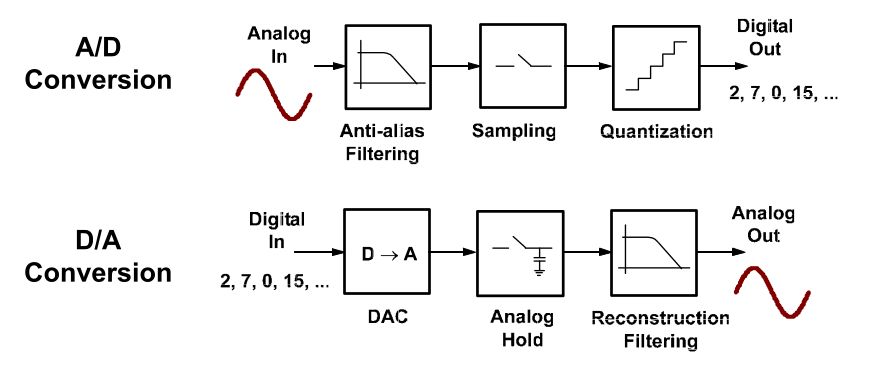
\includegraphics[width=0.8\textwidth]{figs/digital_and_analog_conversion.png}
    \caption{Digital and Analog Conversion}
    \label{fig:digital_analog_conversion}
\end{figure}
\section{Motivation}
Analog-to-Digital Converters (ADCs) and Digital-to-Analog Converters (DACs) provide a link between the Analog world and Digital world. They are essential as information is increalsingly being stored, processed, and transmitted in digital form. The need for high-performance ADCs and DACs is driven by the demand for high-speed data acquisition, signal processing, and communication systems.
physical systems are analog in nature, and the conversion of these signal helps in processing the signal in digital form hence we require D/A conversion interfaces.
Benifits of Digital signal processing
\begin{itemize}
    \item Reduced sensitivity to "analog" noise.
    \item Enhanced functionality and flexibility.
    \item Amenable to automated design \& test.
    \item Direct benefit from the scaling of VLSI technology.
\end{itemize}
\section{Brief History and DACs and ADCs}
Initially, Analog processing was done using analog circuits, but with the advent of digital technology Digital processing has become more prevalent. The first ADCs were developed in the 1950s and 1960s, and they were primarily used in military and aerospace applications. The first DACs were developed in the 1960s, and they were used in audio and video applications. Over the years, the technology has evolved, and today we have high-performance ADCs and DACs that are used in a wide range of applications, including telecommunications, consumer electronics, automotive, and industrial automation.

\section{Objective of the Report}
The objective of this report is to provide a comprehensive understanding of Data Converters in VLSI Systems, focusing on the theoretical aspects of Analog-to-Digital Converters (ADCs) and Digital-to-Analog Converters (DACs). The report aims to explore the principles of operation, design considerations, and performance metrics of these converters. It will also delve into the different CMOS circuits used in ADCs and DACs, including their working principles, advantages, and disadvantages. The report will
also explore research \& advancement Example. NeuADC- An automated design for ADC.


\section{Fundamentals of DACs and ADCs}
\subsection{Digital-to-Analog Converters (DACs)}
Digital-to-Analog Converters (DACs) perform the reverse operation of ADCs by converting discrete digital values into continuous analog signals. They reconstruct the analog signal from the digital input by generating a voltage or current that corresponds to the digital value. The resolution of a DAC is also determined by the number of bits used in the digital input. The performance of a DAC is characterized by parameters such as output voltage range, linearity, settling time, and noise performance.

\subsubsection{DACs Specifications}
The DAC converts an N-bit digital value into a continuous analog voltage, which is a scaled fraction of the reference voltage.
The output voltage (\(V_{out}\)) of a DAC can be expressed as:
\begin{equation}
    V_{out} = V_{REF} \cdot F
\end{equation}
where \(V_{\text{out}}\) is the analog voltage output, \(V_{\text{REF}}\) is the reference voltage, and \(F\) is the fraction defined by the input word, \(D\), that is \(N\) bits wide.
\begin{equation}
    Number\ of\ input\ conditions = 2^N
\end{equation}
F is the fraction of the reference voltage and corresponds to the digital input value \(D\) as follows:
\begin{equation}
    F = \frac{D}{2^N}
\end{equation}
\subsubsection{Specifications of DACs and ADCs}
\begin{itemize}
    \item \textbf{Differential Non-Linearity (DNL):} Measures the deviation of the step size between adjacent digital codes from the ideal value. A high DNL can cause missing codes and degrade performance.
    \item \textbf{Integral Non-Linearity (INL):} Represents the deviation of the actual transfer function from the ideal linear transfer function. It is a critical parameter for accuracy.
    \item \textbf{Offset:} Refers to the difference between the expected output and the actual output when the input is zero. It affects the accuracy of the converter.
    \item \textbf{Latency:} The time delay between the input signal and the corresponding output signal. Lower latency is essential for real-time applications.
    \item \textbf{Signal-to-Noise Ratio (SNR):} The ratio of the signal power to the noise power, indicating the quality of the conversion. Higher SNR values are desirable for better performance.
    \item \textbf{Dynamic Range:} The ratio between the largest and smallest signal levels that the converter can handle. A wide dynamic range is crucial for applications requiring high precision.
\end{itemize}
\subsection{Analog-to-Digital Converters (ADCs)}
Analog-to-Digital Converters (ADCs) are devices that convert continuous analog signals into discrete digital values. They sample the analog signal at regular intervals and quantize the sampled values into a finite number of levels. The resolution of an ADC is determined by the number of bits used to represent the digital output. For example, an 8-bit ADC can represent 256 discrete levels, while a 12-bit ADC can represent 4096 levels. The performance of an ADC is characterized by parameters such as sampling rate, resolution, signal-to-noise ratio (SNR), and total harmonic distortion (THD).
\subsubsection{ADCs Specifications}
DAC is converting a discrete
signal into an analog representation that is also limited by the resolution of the converter,
a fixed number of inputs and outputs are generated. However, with the ADC, the input is
an analog signal with an infinite number of values, which then has to be quantized into an
\(N\)-bit digital word
\begin{equation}
    Number\ of\ Quantizaion\ Levels = 2^N
\end{equation}

\subsection{Types of ADCs and DACs}
\subsubsection{Types of ADCs}
\begin{itemize}
    \item \textbf{Flash ADC:} Uses a resistor ladder network and comparators to convert analog signals to digital instantly. It is fast but consumes more power and area.
    \item \textbf{Successive Approximation Register (SAR) ADC:} Uses a binary search algorithm to approximate the input signal. It is widely used for medium-speed and medium-resolution applications.
    \item \textbf{Sigma-Delta ADC:} Utilizes oversampling and noise shaping to achieve high resolution. Commonly used in audio and precision measurement applications.
    \item \textbf{Pipeline ADC:} Combines multiple stages of ADCs to achieve high speed and resolution. Suitable for high-speed applications like video processing.
    \item \textbf{Dual-Slope ADC:} Measures the input signal by integrating it over a fixed period. It is slow but highly accurate, often used in digital multimeters.
\end{itemize}

\subsubsection{Types of DACs}
\begin{itemize}
    \item \textbf{Binary-Weighted DAC:} Uses resistors weighted in binary values to convert digital signals to analog. It is simple but requires precise resistor values.
    \item \textbf{R-2R Ladder DAC:} Employs a resistor ladder network for conversion. It is efficient and widely used due to its simplicity and scalability.
    \item \textbf{Current Steering DAC:} Converts digital signals to analog by steering currents through different paths. Commonly used in high-speed applications.
    \item \textbf{Sigma-Delta DAC:} Uses oversampling and noise shaping for high-resolution output. Suitable for audio applications.
    \item \textbf{Pulse Width Modulation (PWM) DAC:} Converts digital signals to analog by varying the duty cycle of a pulse. It is simple and cost-effective but requires filtering.
\end{itemize}

\section{Applications of Data Converters}
\begin{itemize}
    \item \textbf{Telecommunications:} Used in modems and communication systems to convert analog signals to digital for processing and vice versa.
    \item \textbf{Consumer Electronics:} Found in devices like smartphones, TVs, and audio systems for signal conversion and processing.
    \item \textbf{Automotive Systems:} Used in sensors and control systems for real-time data acquisition and processing.
    \item \textbf{Medical Devices:} Essential in imaging systems like MRI and CT scans for converting analog signals to digital for analysis.
    \item \textbf{Industrial Automation:} Used in control systems and sensors for monitoring and automation processes.
    \item \textbf{Aerospace and Defense:} Critical in radar systems, communication systems, and signal processing applications.
    \item \textbf{Instrumentation:} Used in digital oscilloscopes, multimeters, and other measurement devices for accurate data acquisition.
\end{itemize}

\subsection{Recent Advancements}


\subsection{issues and Challenges}
\begin{itemize}
    \item \textbf{Design Complexity:} Data converters are challenging to design due to the need for high precision and accuracy, especially with increasing performance requirements.
    \item \textbf{Performance Bottlenecks:} The speed, resolution, or power dissipation of ADCs and DACs can limit the overall system performance, making optimization critical.
    \item \textbf{Scaling Challenges:} As VLSI technology scales down, maintaining performance while reducing area and power consumption becomes increasingly difficult.
    \item \textbf{Noise and Distortion:} Minimizing noise and distortion in high-speed and high-resolution converters is a significant challenge.
    \item \textbf{Cost and Manufacturing Variability:} Achieving high performance while keeping costs low and addressing variability in manufacturing processes is a persistent issue.
\end{itemize}
